\documentclass{article}
\usepackage{tikz}
\usetikzlibrary{graphs,quotes}

\begin{document}

\section*{Structural Causal Models (SCMs)}

\subsection*{Directed Acyclic Graphs (DAGs)}

Structural causal models (SCMs) can be represented as directed acyclic graphs (DAGs), where variables are the nodes and causal effects are represented by directed edges. These graphs encapsulate the causal relationships between variables.

\subsection*{Interventions and Causal Effects}

An intervention is an operation that modifies the structure or behavior of the DAG in some way. Intervening on a variable means erasing the arrows pointing into that variable, setting its value arbitrarily, and then propagating this new value through any directed pathways pointing out from it.

The following diagrams illustrate three different scenarios:
1. On the left, \( X \) is a direct cause of \( Y \); thus, intervening on \( X \) will result in a change in \( Y \).
2. In the middle, there is no direct causal relationship between \( X \) and \( Y \); hence, intervening on \( X \) will not affect \( Y \).
3. On the right, \( X \) influences \( Y \) indirectly via \( Z \); therefore, intervening on \( X \) will still not affect \( Y \).

\subsection*{Example Diagrams}

\begin{figure}[h]
    \centering
    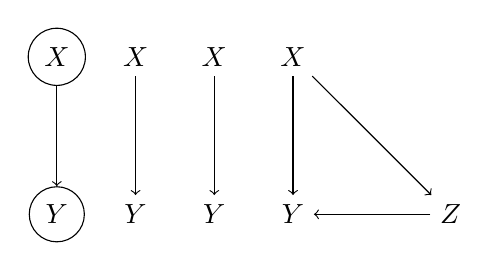
\begin{tikzpicture}
        \begin{scope}[every node/.style={circle, draw}]
            \node (X1) at (0,0) {$X$};
            \node (Y1) at (0,-2) {$Y$};
            
            \draw [->] (X1) -- (Y1);
        \end{scope}
        
        \foreach \x/\y in {1/1,1/2} {
            \begin{scope}[shift={(\x*\y,0)}]
                \node (X\x) at (0,0) {$X$};
                \node (Y\x) at (0,-2) {$Y$};
                
                \draw [->] (X\x) -- (Y\x);
            \end{scope}
        }
        
        \begin{scope}[shift={(3,0)}]
            \node (X3) at (0,0) {$X$};
            \node (Y3) at (0,-2) {$Y$};
            \node (Z3) at (2,-2) {$Z$};
            
            \draw [->] (X3) -- (Y3);
            \draw [->] (X3) -- (Z3);
            \draw [->] (Z3) -- (Y3);
        \end{scope}
    \end{tikzpicture}
    \caption{Three different DAGs representing structural causal models.}
    \label{fig:dags}
\end{figure}

\subsection*{Discussion}

In these examples:
- The left diagram shows a simple direct causal relationship.
- The middle diagram indicates that \( X \) does not directly influence \( Y \).
- The right diagram exhibits a more complex indirect causal relationship where \( X \) affects \( Y \) through an intermediate variable \( Z \).

It is worth noting that the accuracy of some function \( f(X) \) in predicting \( Y \) might be the same across these different scenarios due to the nature of the causal relationships depicted.

\end{document}